% !TeX program = xelatex
\documentclass[runningheads]{llncs}
\usepackage[paperheight=295mm,paperwidth=210mm]{geometry}
\usepackage{graphicx}
\usepackage{wrapfig}
\usepackage{import}
\usepackage{kotex}
\usepackage[dvipsnames]{xcolor}
\usepackage{fancyvrb} %
\usepackage{listings}
\usepackage{tabularx}
\usepackage{underscore}
\usepackage{multicol}
\usepackage{enumitem}
\usepackage{subcaption}
\usepackage[numbers,square,super]{natbib}
\usepackage{mathptmx} % Times New Roman
\usepackage{amsmath}
\usepackage{amssymb}
\usepackage{framed}
\usepackage{etoolbox}
\usepackage{cancel}
\usepackage{physics}
\usepackage{tikz}
\usepackage{parskip}
\usepackage{enumerate}
\usepackage{minted}
\usepackage{inconsolata}
\usepackage{makecell}
\usepackage{slashed}
\usepackage{nicematrix}
\usetikzlibrary{calc, angles, quotes, graphs, positioning, arrows}

\setcounter{tocdepth}{2}

\colorlet{shadecolor}{gray!30}

\newcommand\enclosebox[2]{%
  \BeforeBeginEnvironment{#1}{\begin{#2}}%
  \AfterEndEnvironment{#1}{\end{#2}}%
}

\enclosebox{theorem}{oframed}
\enclosebox{definition}{leftbar}

\newcommand{\divides}{\bigm|}
\newcommand{\ndivides}{%
  \mathrel{\mkern.5mu % small adjustment
    % superimpose \nmid to \big|
    \ooalign{\hidewidth$\big|$\hidewidth\cr$\nmid$\cr}%
  }%
}
\newcommand{\ord}{\operatorname{\mathrm{ord}}}
\newcommand{\ind}{\operatorname{\mathrm{ind}}}
\newcommand{\legendre}[2]{\left(\frac{#1}{#2}\right)}
\setmainfont{Times New Roman}
\setmainhangulfont{Nanum Myeongjo}
\setmonofont{SF Mono}
\setlength{\parindent}{1em}
\setlength{\parskip}{0pt}
\linespread{1.2}
%\renewcommand{\arraystretch}{1.5}
\setlength{\tabcolsep}{0.5em}%
\newenvironment{Figure}
  {\par\medskip\noindent\minipage{\linewidth}}
  {\endminipage\par\medskip}
\newcommand{\translation}[1]{\textsuperscript{#1}}

\makeatletter
\renewcommand\NAT@citesuper[3]{\ifNAT@swa
\if*#2*\else#2\NAT@spacechar\fi
\unskip\kern\p@\textsuperscript{\NAT@@open#1\if*#3*\else,\NAT@spacechar#3\fi\NAT@@close}%
   \else #1\fi\endgroup}
\makeatother

\let\oldtabular\tabular% Store a copy of \tabular
\let\endoldtabular\endtabular% Store a copy of \endtabular
\renewenvironment{tabular}[2][\arraystretch]
  {\edef\arraystretch{#1}% Update \arraystretch
   \oldtabular{#2}}% \begin{tabular}[<stretch>]{<col spec>}
  {\endoldtabular}% \end{tabular}

\begin{document}

\title{Linear Algebra (0031)\newline\space Problem Set 0 Solutions}
\author{Yulwon Rhee (202211342)}
\institute{Department of Computer Science and Engineering, Konkuk University}

\maketitle

% Question 1.
\subsubsection{1.}
(a) Visualise the two vectors $\vb{v}$ and $\vb{w}$ in $\mathbb{R}^2$
\paragraph{Solution.}
\begin{align*}
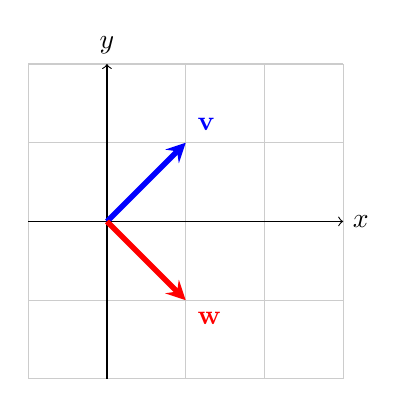
\begin{tikzpicture}
    \draw[thin,gray!40] (-1,-2) grid (3,2);
    \draw[->] (-1,0)--(3,0) node[right]{$x$};
    \draw[->] (0,-2)--(0,2) node[above]{$y$};
    \draw[line width=2pt,blue,-stealth](0,0)--(1,1) node[anchor=south west]{$\vb{v}$};
    \draw[line width=2pt,red,-stealth](0,0)--(1,-1) node[anchor=north west]{$\vb{w}$};
\end{tikzpicture}
\end{align*}

(b) Calculate $\vb{u}=\vb{v}+\vb{w}$, and draw $\vb{u}$ in $\mathbb{R}^2$
\paragraph{Solution.}
$$\vb{u}=\begin{bmatrix}1\\1\end{bmatrix} + \begin{bmatrix}1\\-1\end{bmatrix} = \begin{bmatrix}
    2\\0
\end{bmatrix}$$

\begin{align*}
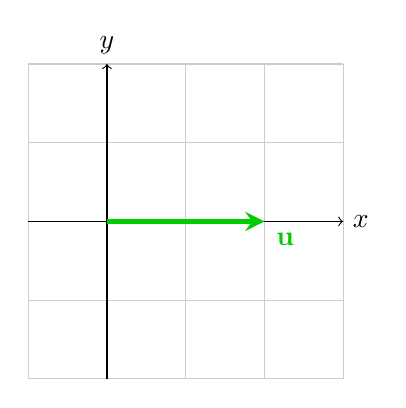
\begin{tikzpicture}
    \draw[thin,gray!40] (-1,-2) grid (3,2);
    \draw[->] (-1,0)--(3,0) node[right]{$x$};
    \draw[->] (0,-2)--(0,2) node[above]{$y$};
    \draw[line width=2pt,black!20!green,-stealth](0,0)--(2,0) node[anchor=north west]{$\vb{u}$};
\end{tikzpicture}
\end{align*}
\newpage
(c) Visualise the operation $\vb{v} + \vb{w}$.
\paragraph{Solution.}
\begin{align*}
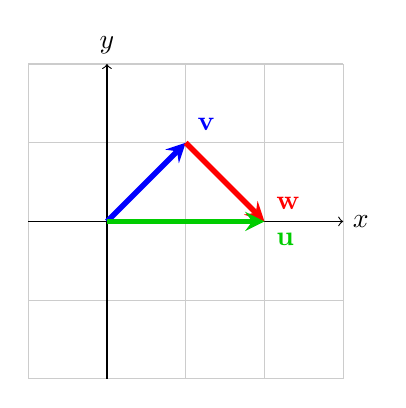
\begin{tikzpicture}
    \draw[thin,gray!40] (-1,-2) grid (3,2);
    \draw[->] (-1,0)--(3,0) node[right]{$x$};
    \draw[->] (0,-2)--(0,2) node[above]{$y$};
    \draw[line width=2pt,blue,-stealth](0,0)--(1,1) node[anchor=south west]{$\vb{v}$};
    \draw[line width=2pt,red,-stealth](1,1)--(2,0) node[anchor=south west]{$\vb{w}$};
    \draw[line width=2pt,black!20!green,-stealth](0,0)--(2,0) node[anchor=north west]{$\vb{u}$};
\end{tikzpicture}
\end{align*}

(d) Visualise the two vectors $2\vb{v}$ and $3\vb{w}$, and also the addition $2\vb{v} + 3\vb{w}$.
\paragraph{Solution.}
\begin{align*}
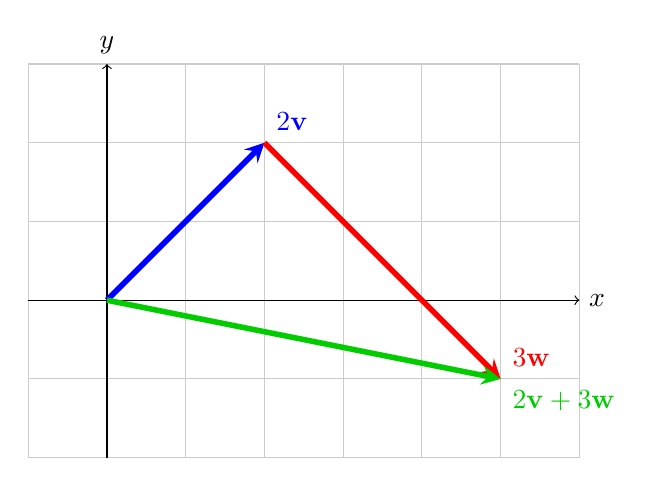
\begin{tikzpicture}
    \draw[thin,gray!40] (-1,-2) grid (6,3);
    \draw[->] (-1,0)--(6,0) node[right]{$x$};
    \draw[->] (0,-2)--(0,3) node[above]{$y$};
    \draw[line width=2pt,blue,-stealth](0,0)--(2,2) node[anchor=south west]{$2\vb{v}$};
    \draw[line width=2pt,red,-stealth](2,2)--(5,-1) node[anchor=south west]{$3\vb{w}$};
    \draw[line width=2pt,black!20!green,-stealth](0,0)--(5,-1) node[anchor=north west]{$2\vb{v}+3\vb{w}$};
\end{tikzpicture}
\end{align*}

(e) Consider $\vb{u} = c\vb{v} + d\vb{w}$. Find an example of $(c, d)$ pair such that $u_1>0, u_2>0$.
\paragraph{Solution.}
\begin{align*}
    \vb{u} &= c\begin{bmatrix}
        1\\1
    \end{bmatrix} + d\begin{bmatrix}
        1\\-1
    \end{bmatrix}\\
    &= \begin{bmatrix}
        c+d\\c-d
    \end{bmatrix}
\end{align*}
example of cases such that $c+d > 0$, $c-d > 0$\\
$$\therefore (c, d) = (1, 0), (2, 1), (2, 0), (3, 2), (3, 1), (3, 0) \cdots$$
\newpage
(f) Repeat part (e) for each of the following cases
\paragraph{Solution.}
\begin{itemize}
    \item $u_1 > 0,\ u_2 < 0$
    \begin{gather*}
        c+d > 0,\ c-d < 0\\
        \therefore (c, d) = (0, 1), (0, 2), (0, 3), (1, 2), (1, 3), (2, 3) \cdots
    \end{gather*}
    \item $u_1 < 0,\ u_2 > 0$
    \begin{gather*}
        c+d < 0,\ c-d > 0\\
        \therefore (c, d) = (-1, -2), (-1, -3), (-1, -4), (-2, -3), (-2, -4), (-2, -5) \cdots
    \end{gather*}
    \item $u_1 < 0,\ u_2 < 0$
    \begin{gather*}
        c+d < 0,\ c-d < 0\\
        \therefore (c, d) = (-1, 0), (-2, -1), (-2, 0), (-3, -2), (-3, -1), (-3, 0) \cdots    
    \end{gather*}
\end{itemize}

(g) Do you think you can get any point in $\mathbb{R}^2$ with the linear combination $c\vb{v}+d\vb{w}$? Justify your answer.
\paragraph{Solution.}
$$\alpha = \frac{1}{2},\ \beta = \frac{1}{2}\quad\longrightarrow\quad\alpha\vb{v}+\beta\vb{w} = \begin{bmatrix}
    1\\0
\end{bmatrix}$$
$$\gamma = \frac{1}{2},\ \delta = -\frac{1}{2}\quad\longrightarrow\quad\gamma\vb{v}+\delta\vb{w} = \begin{bmatrix}
    0\\1
\end{bmatrix}$$
Since $c\begin{bmatrix}
    1\\0
\end{bmatrix} + d\begin{bmatrix}
    0\\1
\end{bmatrix}$ can represent any point in $\mathbb{R}^2$, $c\vb{v}+d\vb{w}$ can also represent any point in $\mathbb{R}^2$.\qed
\newpage
(h) Answer the same question in part (g) with new vectors $\vb{v}=\begin{bmatrix}
    1\\-2
\end{bmatrix}$ and $\vb{w}=\begin{bmatrix}
    -2\\4
\end{bmatrix}$
\paragraph{Solution.}
There's no real root for $c\vb{v}+d\vb{w}=\begin{bmatrix}
    1\\0
\end{bmatrix}$ or $\begin{bmatrix}
    0\\1
\end{bmatrix}$.\\
Also,
\begin{gather*}
    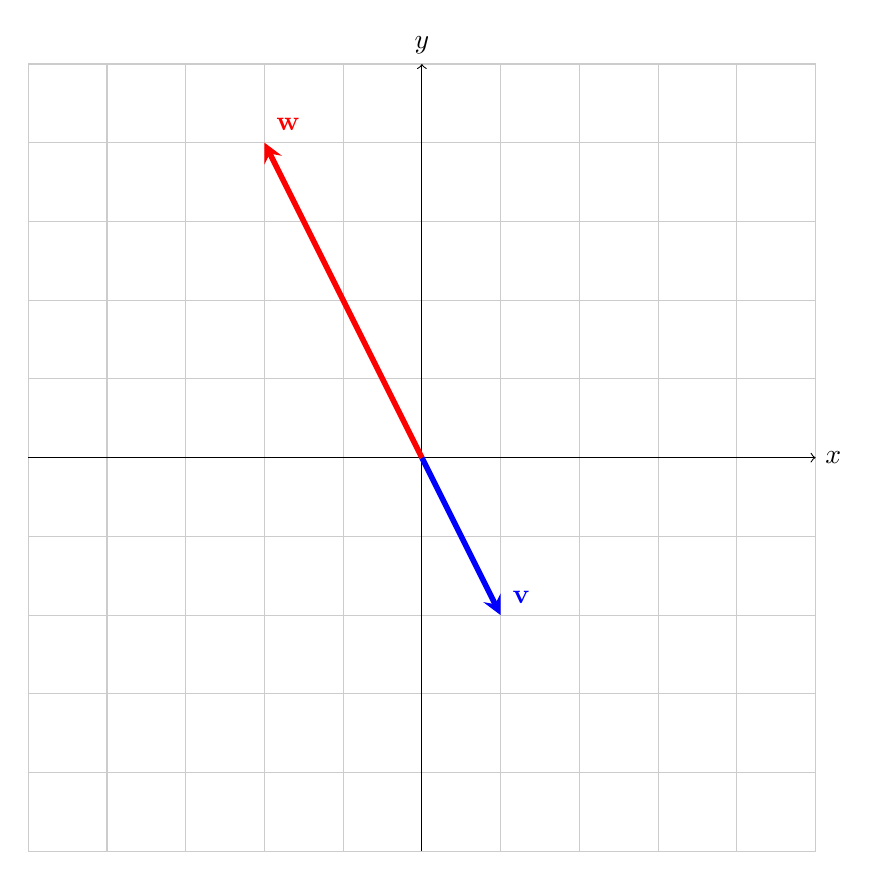
\begin{tikzpicture}
        \draw[thin,gray!40] (-5,-5) grid (5,5);
        \draw[->] (-5,0)--(5,0) node[right]{$x$};
        \draw[->] (0,-5)--(0,5) node[above]{$y$};
        \draw[line width=2pt,blue,-stealth](0,0)--(1,-2) node[anchor=south west]{$\vb{v}$};
        \draw[line width=2pt,red,-stealth](0,0)--(-2,4) node[anchor=south west]{$\vb{w}$};
    \end{tikzpicture}
\end{gather*}
As you can see, the linear combination of $\vb{v}$ and $\vb{w}$ can represent only points on the $y=-2x$.
So, $c\vb{v}+d\vb{w}$ cannot represent any point in $\mathbb{R}^2$. \qed
\newpage
\subsubsection{2.}
(a) Visualise $c\begin{bmatrix}
    1\\0
\end{bmatrix}+d\begin{bmatrix}
    0\\1
\end{bmatrix}$ for all scalars $c, d$.
\paragraph{Solution.}
\begin{align*}
    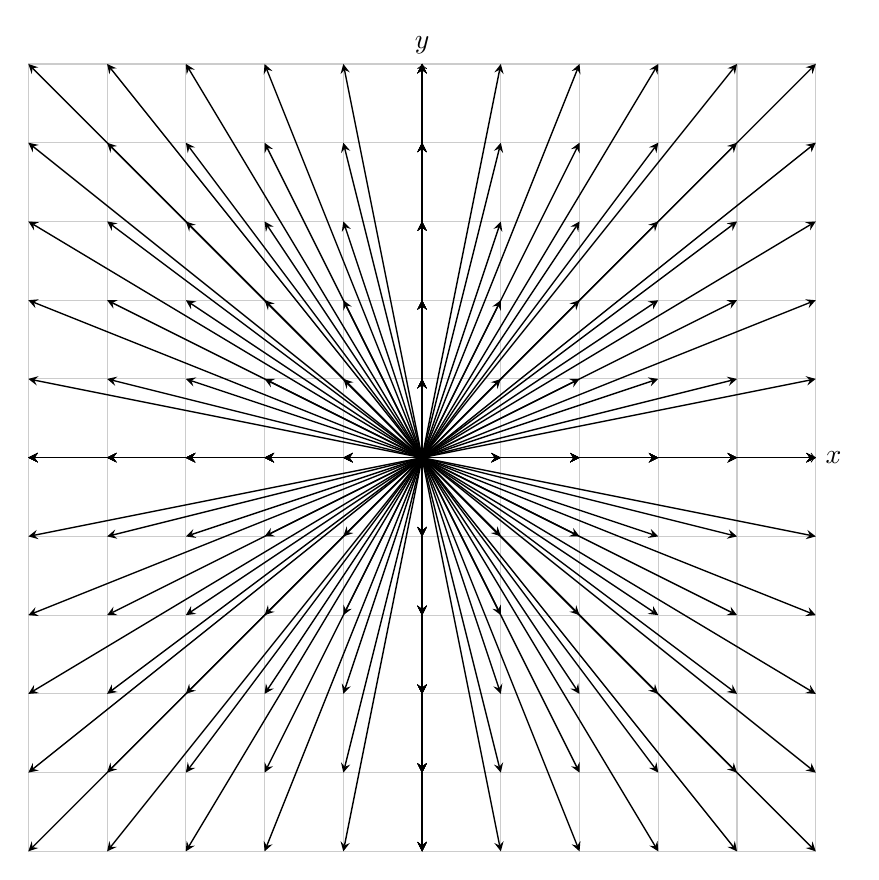
\begin{tikzpicture}
        \draw[thin,gray!40] (-5,-5) grid (5,5);
        \draw[->] (-5,0)--(5,0) node[right]{$x$};
        \draw[->] (0,-5)--(0,5) node[above]{$y$};
        \foreach \x in {0, ..., 5} {
            \foreach \y in {0, ..., 5} {
                \draw[line width=0.5pt,black,-stealth](0,0)--(\x, \y);
                \draw[line width=0.5pt,black,-stealth](0,0)--(\x, 0);
                \draw[line width=0.5pt,black,-stealth](0,0)--(0, \y);
                \draw[line width=0.5pt,black,-stealth](0,0)--(\x, -\y);
                \draw[line width=0.5pt,black,-stealth](0,0)--(-\x, 0);
                \draw[line width=0.5pt,black,-stealth](0,0)--(-\x, \y);
                \draw[line width=0.5pt,black,-stealth](0,0)--(-\x, -\y);
                \draw[line width=0.5pt,black,-stealth](0,0)--(0, -\y);
            }
        }
    \end{tikzpicture}
\end{align*}
Drawn all $c\begin{bmatrix}
    1\\0
\end{bmatrix}+d\begin{bmatrix}
    0\\1
\end{bmatrix} (c, d \in \mathbb{Z}, -5 \leq c, d\leq 5)$.
\begin{align*}
    \therefore c\begin{bmatrix}
        1\\0
    \end{bmatrix}+d\begin{bmatrix}
        0\\1
    \end{bmatrix} = \begin{bmatrix}
        c\\d
    \end{bmatrix} \in \mathbb{R}^2\quad(\because c, d \in \mathbb{R})
\end{align*}

(b) Consider $\vb{v} = \begin{bmatrix}
    1\\2
\end{bmatrix}$ and $\vb{w} = \begin{bmatrix}
    2\\1
\end{bmatrix}$. Express $\vb{v}$ and $\vb{w}$ as a linear combination of $\begin{bmatrix}
    1\\0
\end{bmatrix}$ and $\begin{bmatrix}
    0\\1
\end{bmatrix}$.
\paragraph{Solution.}
\begin{align*}
    \vb{v} = \begin{bmatrix}
        1\\0
    \end{bmatrix} + 2\begin{bmatrix}
        0\\1
    \end{bmatrix}\\
    \vb{w} = 2\begin{bmatrix}
        1\\0
    \end{bmatrix} + \begin{bmatrix}
        0\\1
    \end{bmatrix}
\end{align*}
\newpage
(c) Visualise $c\vb{v}+d\vb{w}$ for all $c, d$.
\paragraph{Solution.}
\begin{align*}
    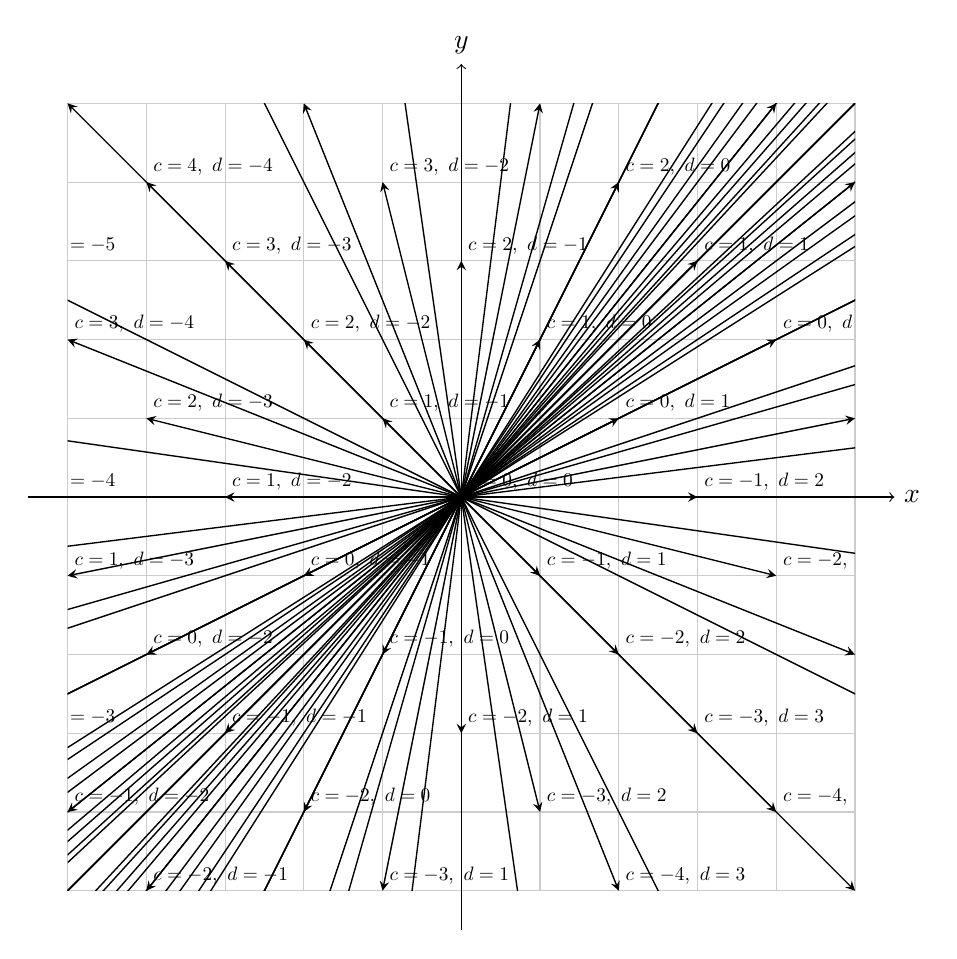
\begin{tikzpicture}
        \draw[thin,gray!40] (-5,-5) grid (5,5);
        \draw[->] (-5.5,0)--(5.5,0) node[right]{$x$};
        \draw[->] (0,-5.5)--(0,5.5) node[above]{$y$};
        \begin{scope}
            \clip (-5,-5) rectangle (5,5);
            \foreach \c/\sc in {-5, ..., 5} {
                \foreach \d/\sd in {-5, ..., 5} {
                    \pgfmathsetmacro\x{\c + \d * 2}
                    \pgfmathsetmacro\y{\c * 2 + \d}
                    \draw[line width=0.5pt,black,-stealth](0,0)--(\x, \y) node[anchor=south west, scale=0.7]{$c=\c,\ d=\d$};
                }
            }
        \end{scope}
    \end{tikzpicture}
\end{align*}
Drawn all $c\vb{v}+d\vb{w} (c, d \in \mathbb{Z}, -5 \leq c, d\leq 5)$ .
\subsubsection{3.}
(a) Calculate $A + B$ for $A = \begin{bmatrix}
    0 & -3 & 1 \\
    5 & 7 & -4 \\
    3 & -1 & -3 \\
    7 & -1 & 9
\end{bmatrix},\ B = \begin{bmatrix}
    5 & 4 & -3 \\
    2 & 1 & 8 \\
    -3 & 7 & 10 \\
    2 & -4 & -2
\end{bmatrix}$.
\paragraph{Solution.}
$$A + B = \begin{bmatrix}
    0 & -3 & 1 \\
    5 & 7 & -4 \\
    3 & -1 & -3 \\
    7 & -1 & 9
\end{bmatrix} + \begin{bmatrix}
    5 & 4 & -3 \\
    2 & 1 & 8 \\
    -3 & 7 & 10 \\
    2 & -4 & -2
\end{bmatrix} = \begin{bmatrix}
    5 & 1 & -2 \\
    7 & 8 & 4 \\
    0 & 6 & 7 \\
    9 & -5 & -7
\end{bmatrix}$$

(b) Let $A = \begin{bmatrix}
    a & -5\\
    -3 & c\\
    e & 4
\end{bmatrix}$ and $B = \begin{bmatrix}
    5 & b\\
    d & -7\\
    6 & f
\end{bmatrix}$. Find the values of $a, b, c, d, e, f$ so that $$3A + 2B = \begin{bmatrix}
    5 & 10\\
    15 & 1\\
    11 & 30
\end{bmatrix}$$
\paragraph{Solution.}
\begin{align*}
    3A + 2B &= \begin{bmatrix}
        3a & -15\\
        -9 & 3c\\
        3e & 12
    \end{bmatrix} + \begin{bmatrix}
        10 & 2b\\
        2d & -14\\
        12 & 2f
    \end{bmatrix}\\
    &=\begin{bmatrix}
        3a + 10 & 2b - 15\\
        2d - 9 & 3c - 14\\
        3e + 12 & 2f + 12
    \end{bmatrix}\\
    &=\begin{bmatrix}
        5 & 10\\
        15 & 1\\
        11 & 30
    \end{bmatrix}\\
\end{align*}
from above,
\begin{gather*}
    \begin{cases}
        3a+10 = 5\\2b - 15 = 10\\3c - 14 = 1\\2d - 9 = 15\\3e + 12 = 11\\2f + 12 = 30
    \end{cases}\\\\
    \therefore a = -\frac{5}{3},\quad b = \frac{25}{2},\quad c = 5,\quad d = 12,\quad e = -\frac{1}{3},\quad f = 9
\end{gather*}
\newpage
(c) Find the two matrices $A$ and $B$ that satisfy $A + B = \begin{bmatrix}
    3&7\\1&-6
\end{bmatrix}$ and $A - B = \begin{bmatrix}
    9&-4\\-5&-9
\end{bmatrix}$.
\paragraph{Solution.}

\begin{gather*}
    (A + B) + (A - B) = 2A = \begin{bmatrix}
        12&3\\-4&-15
    \end{bmatrix}\\
    \therefore A = \begin{bmatrix}
        6 & \frac{3}{2}\\
        -2&-\frac{15}{2}
    \end{bmatrix}\\\\
    (A + B) - (A - B) = 2B = \begin{bmatrix}
        -6&11\\6&3
    \end{bmatrix}\\
    \therefore B = \begin{bmatrix}
        -3 & \frac{11}{2}\\
        3&-\frac{3}{2}
    \end{bmatrix}
\end{gather*}

\subsubsection{4.}
(a) Calculate the inner product $\vb{a}\cdot\vb{b}$.
\paragraph{Solution.}
\begin{align*}
    \vb{a}\cdot\vb{b} &= \begin{bmatrix}
        2\\1\\2\\1
    \end{bmatrix} \cdot \begin{bmatrix}
        2\\1\\2\\6
    \end{bmatrix}\\&= 2 \times 2 + 1 \times 1 + 2 \times 2 + 1 \times 6\\&= 4 + 1 + 4 + 6\\&= 15
\end{align*}

(b) Calculate $||\vb{a}||$ and $||\vb{b}||$.
\paragraph{Solution.}
\begin{align*}
    ||\vb{a}|| &= \sqrt{2^2 + 1^2 + 2^2 + 1^2}\\&= \sqrt{4 + 1 + 4 + 1}\\&= \sqrt{10}\\
    ||\vb{b}|| &= \sqrt{2^2 + 1^2 + 2^2 + 6^2}\\&= \sqrt{4 + 1 + 4 + 36}\\&= \sqrt{45}\\&= 3\sqrt{5}
\end{align*}
\newpage
(c) Calculate the angle (ranging from $0$ to $\pi$) between $\vb{a}$ and $\vb{b}$.
\paragraph{Solution.}
\begin{align*}
    15 = 15 \sqrt{2}\cos\theta\quad(\because \vb{a} \cdot \vb{b} &= ||\vb{a}||\cdot||\vb{b}||\cos\theta)\\
    \cos\theta = \frac{1}{\sqrt{2}}\\
    \therefore \theta = \frac{\pi}{4} \quad(\because 0 \leq \theta \leq \pi)
\end{align*}

\subsubsection{5.}
(a) Expand $||\vb{v} + \vb{w}||^2$.
\paragraph{Solution.}
\begin{align*}
    ||\vb{v} + \vb{w}||^2 = ||\vb{v}||^2 + 2\vb{v}\cdot\vb{w} + ||\vb{w}||^2
\end{align*}

(b) Expand $(||\vb{v}||+||\vb{w}||)^2$.
\paragraph{Solution.}
\begin{align*}
    (||\vb{v}|| + ||\vb{w}||)^2 = ||\vb{v}||^2 + 2||\vb{v}||\cdot||\vb{w}|| + ||\vb{w}||^2
\end{align*}

(c) Use the results in parts (a) and (b) to show the triangle inequality.
\paragraph{Solution.}
By the Cauchy-Schwarz Inequality, $$\vb{v}\cdot\vb{w} \leq ||\vb{v}||\cdot||\vb{w}||$$
So, $$||\vb{v} + \vb{w}||^2 = ||\vb{v}||^2 + 2\vb{v}\cdot\vb{w} + ||\vb{w}||^2\leq||\vb{v}||^2 + 2||\vb{v}||\cdot||\vb{w}|| + ||\vb{w}||^2 = (||\vb{v}|| + ||\vb{w}||)^2$$
i.e., \begin{align*}
    ||\vb{v} + \vb{w}||^2\leq(||\vb{v}|| + ||\vb{w}||)^2 \ \Longrightarrow\ ||\vb{v} + \vb{w}|| \leq ||\vb{v}|| + ||\vb{w}||
    \tag*{$\qed$}
\end{align*}

\subsubsection{6.}
(a) Prove that $-1\leq\frac{\vb{v}\cdot\vb{w}}{||\vb{v}||\cdot||\vb{w}||}\leq1$.
\paragraph{Solution 1.}
By the Cauchy-Schwarz Inequality,
\begin{gather*}
    |\vb{v}\cdot\vb{w}|\leq||\vb{v}||\cdot||\vb{w}||\\
    \frac{|\vb{v}\cdot\vb{w}|}{||\vb{v}||\cdot||\vb{w}||}\leq1\\
    \therefore -1\leq\frac{\vb{v}\cdot\vb{w}}{||\vb{v}||\cdot||\vb{w}||}\leq1\tag*{$\qed$}
\end{gather*}
\paragraph{Solution 2.}
\begin{align*}
    \frac{\vb{v}\cdot\vb{w}}{||\vb{v}||\cdot||\vb{w}||}&= \frac{||\vb{v}||\cdot||\vb{w}||\cos\theta}{||\vb{v}||\cdot||\vb{w}||}\\&= \cos\theta\\
    -1 \leq \cos\theta \leq 1\tag*{$\qed$}
\end{align*}

(b), (c) Let $\vb{v}=\begin{bmatrix}
    a\\b
\end{bmatrix}$ and $\vb{w} = \begin{bmatrix}
    1\\1
\end{bmatrix}$ with $a^2+b^2=2$. Find the vector $\vb{v}$ for each of the following cases, and visualise the vectors $\vb{w}$, and $\vb{v}$.
\paragraph*{Solution.}
\begin{enumerate}[i.]
    \item $\frac{\vb{v}\cdot\vb{w}}{||\vb{v}||\cdot||\vb{w}||} = 1$\\
    \begin{gather*}
        \frac{\vb{v}\cdot\vb{w}}{||\vb{v}||\cdot||\vb{w}||} = \cos\theta = 1\\\therefore\theta = 0
    \end{gather*}
    \begin{gather*}
        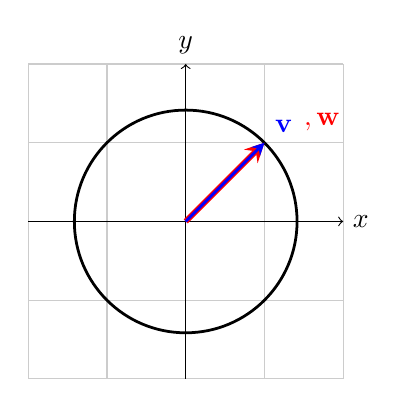
\begin{tikzpicture}
            \coordinate (O) at (0,0);
            \draw[thin,gray!40] (-2,-2) grid (2,2);
            \draw[->] (-2,0)--(2,0) node[right]{$x$};
            \draw[->] (0,-2)--(0,2) node[above]{$y$};
            \draw[black, line width=1pt] (0,0) circle (1.414213); %node[anchor=south east]{$x^2+y^2=2$};
            \draw[line width=2pt,red,-stealth](0,0)--(1,1) node[anchor=south west]{$\quad,\vb{w}$};
            \draw[line width=1pt,blue,-stealth](0,0)--(1,1) node[anchor=south west]{$\vb{v}$};
        \end{tikzpicture}\\
        \therefore \vb{v} = \begin{bmatrix}
            1\\1
        \end{bmatrix}
    \end{gather*}
    \\\\\\\\\\\\\\\\\\\\\\\\
    \item $\frac{\vb{v}\cdot\vb{w}}{||\vb{v}||\cdot||\vb{w}||} = \frac{1}{\sqrt{2}}$\\
    \begin{gather*}
        \frac{\vb{v}\cdot\vb{w}}{||\vb{v}||\cdot||\vb{w}||} = \cos\theta = \frac{1}{\sqrt{2}}\\
        \therefore\theta=\frac{\pi}{4}
    \end{gather*}
    \begin{gather*}
        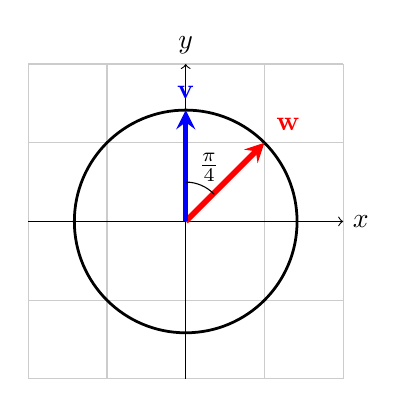
\begin{tikzpicture}
            \coordinate (O) at (0,0);
            \draw[thin,gray!40] (-2,-2) grid (2,2);
            \draw[->] (-2,0)--(2,0) node[right]{$x$};
            \draw[->] (0,-2)--(0,2) node[above]{$y$};
            \draw[black, line width=1pt] (0,0) circle (1.414213); %node[anchor=south east]{$x^2+y^2=2$};
            \draw[line width=2pt,red,-stealth](0,0)--(1,1) node(w)[anchor=south west]{$\vb{w}$};
            \draw[line width=2pt,blue,-stealth](0,0)--(0,1.414213) node(v)[anchor=south]{$\vb{v}$};
            \pic [draw, "$\frac{\pi}{4}$", angle eccentricity=1.5] {angle = w--O--v};
        \end{tikzpicture}\\
        \therefore \vb{v} = \begin{bmatrix}
            0\\\sqrt{2}
        \end{bmatrix}
    \end{gather*}
    \item $\frac{\vb{v}\cdot\vb{w}}{||\vb{v}||\cdot||\vb{w}||} = 0$\\
    \begin{gather*}
        \frac{\vb{v}\cdot\vb{w}}{||\vb{v}||\cdot||\vb{w}||} = \cos\theta = 0\\
        \therefore\theta=\frac{\pi}{2}
    \end{gather*}
    \begin{gather*}
        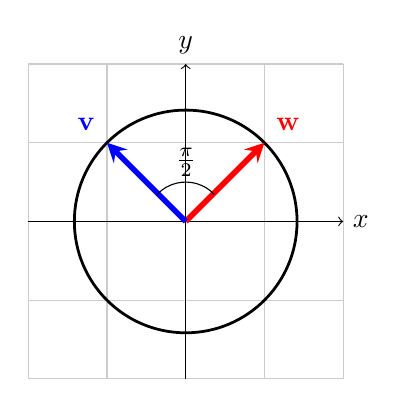
\begin{tikzpicture}
            \coordinate (O) at (0,0);
            \draw[thin,gray!40] (-2,-2) grid (2,2);
            \draw[->] (-2,0)--(2,0) node[right]{$x$};
            \draw[->] (0,-2)--(0,2) node[above]{$y$};
            \draw[black, line width=1pt] (0,0) circle (1.414213); %node[anchor=south east]{$x^2+y^2=2$};
            \draw[line width=2pt,red,-stealth](0,0)--(1,1) node(w)[anchor=south west]{$\vb{w}$};
            \draw[line width=2pt,blue,-stealth](0,0)--(-1,1) node(v)[anchor=south east]{$\vb{v}$};
            \pic [draw, "$\frac{\pi}{2}$", angle eccentricity=1.5] {angle = w--O--v};
        \end{tikzpicture}\\
        \therefore \vb{v} = \begin{bmatrix}
            -1\\1
        \end{bmatrix}
    \end{gather*}
    \item $\frac{\vb{v}\cdot\vb{w}}{||\vb{v}||\cdot||\vb{w}||} = -\frac{1}{\sqrt{2}}$\\
    \begin{gather*}
        \frac{\vb{v}\cdot\vb{w}}{||\vb{v}||\cdot||\vb{w}||} = \cos\theta = -\frac{1}{\sqrt{2}}\\
        \therefore\theta=\frac{3}{4}\pi
    \end{gather*}
    \begin{gather*}
        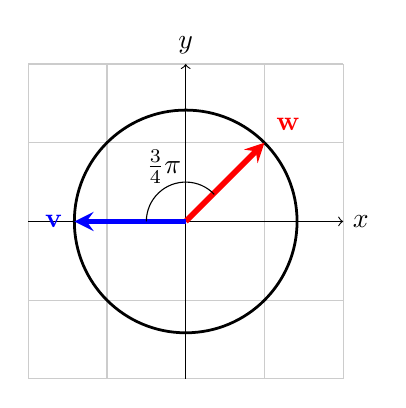
\begin{tikzpicture}
            \coordinate (O) at (0,0);
            \draw[thin,gray!40] (-2,-2) grid (2,2);
            \draw[->] (-2,0)--(2,0) node[right]{$x$};
            \draw[->] (0,-2)--(0,2) node[above]{$y$};
            \draw[black, line width=1pt] (0,0) circle (1.414213); %node[anchor=south east]{$x^2+y^2=2$};
            \draw[line width=2pt,red,-stealth](0,0)--(1,1) node(w)[anchor=south west]{$\vb{w}$};
            \draw[line width=2pt,blue,-stealth](0,0)--(-1.414213,0) node(v)[anchor=east]{$\vb{v}$};
            \pic [draw, "$\frac{3}{4}\pi$", angle eccentricity=1.5] {angle = w--O--v};
        \end{tikzpicture}\\
        \therefore \vb{v} = \begin{bmatrix}
            -\sqrt{2}\\0
        \end{bmatrix}
    \end{gather*}
    \item $\frac{\vb{v}\cdot\vb{w}}{||\vb{v}||\cdot||\vb{w}||} = -1$\\
    \begin{gather*}
        \frac{\vb{v}\cdot\vb{w}}{||\vb{v}||\cdot||\vb{w}||} = \cos\theta = -1\\
        \therefore\theta=\pi
    \end{gather*}
    \begin{gather*}
        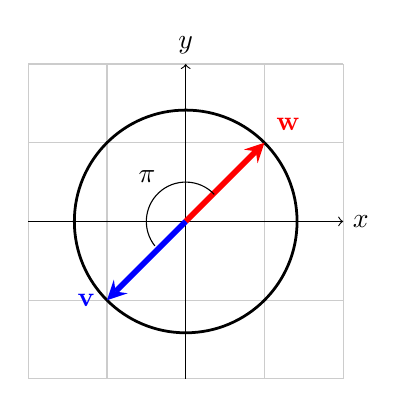
\begin{tikzpicture}
            \coordinate (O) at (0,0);
            \draw[thin,gray!40] (-2,-2) grid (2,2);
            \draw[->] (-2,0)--(2,0) node[right]{$x$};
            \draw[->] (0,-2)--(0,2) node[above]{$y$};
            \draw[black, line width=1pt] (0,0) circle (1.414213); %node[anchor=south east]{$x^2+y^2=2$};
            \draw[line width=2pt,red,-stealth](0,0)--(1,1) node(w)[anchor=south west]{$\vb{w}$};
            \draw[line width=2pt,blue,-stealth](0,0)--(-1,-1) node(v)[anchor=east]{$\vb{v}$};
            \pic [draw, "$\pi$", angle eccentricity=1.5] {angle = w--O--v};
        \end{tikzpicture}\\
        \therefore \vb{v} = \begin{bmatrix}
            -1\\-1
        \end{bmatrix}
    \end{gather*}
\end{enumerate}
\newpage
(d) Use the results in parts (b) and (c) to argue that the value $\frac{\vb{v}\cdot\vb{w}}{||\vb{v}||\cdot||\vb{w}||}$ is an appropriate metric for representing "similarity" of two vectors in some sense.
\paragraph*{Solution.}
By the $\cos\theta$ value of the angle between two vectors can represent the similarity of two vectors.
e.g. $cosine\ similarity$ of two identical vectors is equal to $1$.
And $cosine\ similarity$ between $\vb{v}$ and $-\vb{v}$(the angle is totally different) is equal to -1.
As the angle of the two vectors increases from $0$ to $\pi$, the $cosine\ similarity$ value goes to $-1$ from $1$ CONTINUOUSLY as shown in (c).
Therefore, I think it can be useful when representing the difference between two data.


\end{document}